%%%%%%%%%%%%%%%%%%%%%%% file pestova.tex %%%%%%%%%%%%%%%%%%%%%%%%%
%
% Toto je zdrojovy subor LaTeXu, ktory treba pouzit ako sablonu pre vas  
% clanok - nakopirujte ho do noveho suboru VASE 'priezvisko.tex' 
% a zmodifikujte.
%
% Clanok musi byt napisany po anglicky v zakladnom kode ASCII s medzinarodnym kodovanim akcentov
% teda nesmie byt pouzity \usepackage{slovak}.
%
% Subor 'priezvisko.tex' a vsetky obrazky (jpg, png, alebo pdf) pouzite v prostredi figures
% musia byt umiestnene v podadresari 'priezvisko' adresara 'template'. 
%
% POUZIVAJTE medzinarodne akcenty, teda \"a namiesto (�), \'a namiesto (�), \v{c} namiesto (�), \softL namiesto (�), ...
% Teda NEMOZNO POUZIVAT PRIAMO �iadny makcen, dlzen, apod !!!!!!!!!!
% NEMOZNO pridavat ani ziadne dalsie baliky, a to ani do suboru priezvisko.tex, ani do hlavneho suboru template.tex
% teda nesmie byt doplneny ziadny z tychto dvoch suborov o
% \usepackage{....}
%%%%%%%%%%%%%%%%%%%%%%%%%%%%%%%%%%%%%%%%%%%%%%%%%%%%%%%%%%%%%%%%%%%

% NIZSIE TREBA POZORNE A DOSLEDNE PONAHRADZAT TOTO:

% NAHRADTE TENTO NAZOV VLASTNYM UPLNYM NAZVOM SVOJHO CLANKU
\title{IPFIX Mediation Framework of the SLAmeter Tool}

% NAHRADTE TENTO SKRATENY NAZOV SKRATENYM NAZVOM SVOJHO CLANKU
\titlerunning{IPFIX Mediation Framework}

% NAHRADTE AUTOROV (s plnymi menami a priezviskami, medzinarodne kodovane a oddelene pomocou \and
\author{Rastislav Kudla \and Peter Feci\softl ak \and Adri\'an Pek\'ar}

% NAHRADTE OPAT AUTOROV (s inicialami mien a priezviskami, medzinarodne kodovane a oddelene pomocou \and
\authorrunning{R. Kudla \and P. Feci\softl ak \and A. Pek\'ar}

% TOTO NEMENTE
\institute{Department of Computers and Informatics\\
Technical University of Ko\v{s}ice, Letn\'a 9, 042 00 Ko\v{s}ice, Slovakia\\
% OR ADD another institute
% \and
% Other Institute\\
}

%% OPATOVNE NAHRADTE UPLNY NAZOV CLANKU A AUTOROV S UPLNYMI MENAMI,
%% ALE TENTOKRAT ICH NEODDELUJTE pomocou \and, ale iba pomocou and (teda bez spatnej lomky)
%% na zaklade nasledujucich dvoch riadkov totiz sa dostanu informacie o nazve a autoroch
%% do obsahu zbornika (to contents)
\toctitle{IPFIX Mediation Framework of the SLAmeter Tool}
\tocauthor{Rastislav Kudla, Peter Feci\softl ak and Adri\'an Pek\'ar}
\maketitle

%%%%%%%%%%%%%%%%%%%%%%%%%%%%%%%%%%%%%%%%%%%%%%%%%%%%%%%%%%%%%%%%%%%%%%%%%%%%%%%%%%
% A TERAZ MOZETE MODIFIKOVAT NASLEDUJUCI OBSAH PODLA OBSAHU SVOJHO CLANKU
% ACKNOWLEDGEMENT nechajte tak ako je, ak vam vas veduci nepovie inak. 
%

\begin{abstract}
Presented paper deals with the IP Flow Information Export (IPFIX) Mediation Problem. 
The problem was elaborated by IPFIX working group in RFC~5982 and RFC~6183.
The aim of this work is to design and implement an IPFIX Mediation Framework of the 
SLAmeter monitoring tool based on these documents. 
The analytical part is devoted to the IPFIX Mediation Problem. The core part of the paper 
is represented by the design and description of~implementation workflow of~IPFIX Mediation Framework. 
The main contribution of this work is to extend the possibilities of monitoring application SLAmeter.

\keywords{IPFIX, Mediation, Mediator, Collector, Exporter, SLAmeter, BasicMeter, MONICA}
\end{abstract}


\section{Introduction}

The trend of recent years in computer networking are converged networks which combine data, 
voice and video transmission into one common infrastructure. However, with increasing growth 
of~opportunities raises demand for~quality. In~order~to compare or even increase quality 
of~networks and service, it is necessary to have the ability to measure network parameters.

SLAmeter is measuring architecture being developed by the MONICA research group in Computer 
Networks Laboratory at the Technical University of Ko\v{s}ice. It is a tool for passive 
flow-based measurement and subsequent network traffic analysis with the purpose of determining 
the grade of network quality \cite{slameter}.

Flow-based measurement is a popular method for various network
monitoring usages. The sharing of flow-based information for
monitoring applications having different requirements raises some
open issues in terms of measurement system scalability and capacity, flow-based
measurement flexibility, and export reliability. \emph{IP Flow
Information Export (IPFIX) Mediation} may help resolve these issues \cite{rfc5982}.

\section{Motivation}

To fulfil application requirements with limited system resources, the IPFIX architecture needs to 
introduce an intermediate entity between Exporters and Collectors. From a data manipulation point of 
view, this intermediate entity may provide the aggregation, correlation, filtering, and modification of 
Flow Records to save measurement system resources and to perform preprocessing tasks for the Collector. 
From a protocol conversion point of view, this intermediate entity may provide conversion into IPFIX, 
or conversion of IPFIX transport protocols (e.g., from unreliable, connectionless UDP to the 
Stream Control Transmission Protocol (SCTP)) to improve the export reliability \cite{rfc6183}. 


\section{Goals}

The aim of this work is to analyse, design, implement and test an framework for 
intermediate entity (Mediator) between exporter and collector in the IPFIX protocol.
This work also integrates the solution with the existing architecture of the SLAmeter monitoring 
tool. Framework put a great emphasis on its modularity in order to make it easy and convenient 
to implement new mediation modules and thereby increase monitoring possibilities of SLAmeter.

\section{Analysis}

\subsection{Terminology and Definitions}

The IPFIX-specific terminology used in this paper is defined in \cite{rfc5101}.  Let us define 
the IPFIX Mediation-specific terms here.

\begin{itemize}
 \item \textbf{Record stream} -- a stream of records carrying flow-based information. The records are
 encoded as IPFIX Data Records.
 
 \item \textbf{IPFIX Mediation} -- the manipulation and conversion of a record stream for subsequent 
 export using the IPFIX protocol.
 
 \item \textbf{Intermediate Process} -- takes a record stream as its input from Collecting Processes, 
 or other Intermediate Processes performs some transformations on this stream, based 
 upon the content of each record and passes the transformed record stream as its output to Exporting 
 Processes, or other Intermediate Processes, in order to perform IPFIX Mediation.
 
 \item \textbf{IPFIX Mediator} is an IPFIX Device that provides IPFIX Mediation by receiving a record 
 stream from IPFIX Exporter or other Mediator, hosting one or more Intermediate Processes to transform 
 that stream, and exporting the transformed record stream to IPFIX Collector via IPFIX Messages. \cite{rfc5982}
 \end{itemize}
 
 Fig.~\ref{o:eng_exp-med-coll} depicts one of the possible IPFIX Exporter -- Mediator -- Collector 
 architecture examples.
\begin{figure}[ht!]
\centering
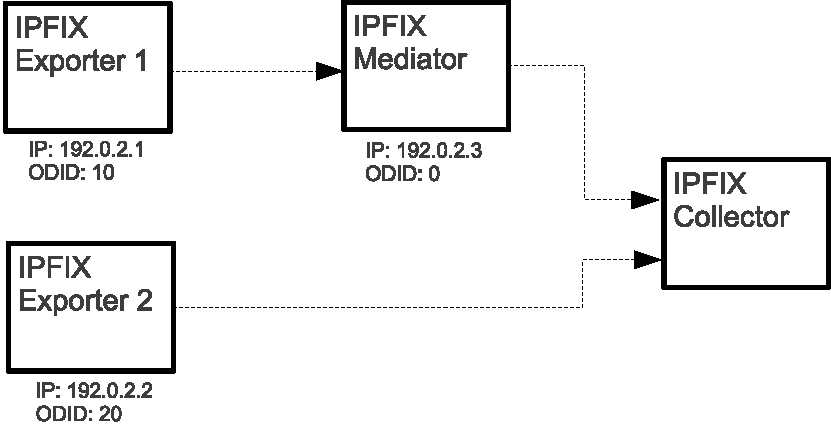
\includegraphics[width=0.7\textwidth]{kudla/eng_exp-med-coll}
\caption{One of the possible IPFIX Exporter -- Mediator -- Collector architecture examples}\label{o:eng_exp-med-coll}
\end{figure}

\subsection{Problem statement}

Network administrators generally face the problems of measurement system scalability, flow-based 
measurement flexibility, and export reliability, even if some techniques, such as Packet Sampling,
Filtering, Data Records aggregation, and export replication, have already been developed.  

The problems consist of adjusting some parameters of metering devices to resources of the measurement 
system while fulfilling appropriate conditions: data accuracy, flow granularity, and export reliability. 
These conditions depend on two factors -- \textbf{measurement system capacity} and 
\textbf{application requirements}.

Due to resource limitations of the measurement system, it is important to use traffic data reduction 
techniques as early as possible, e.g., at the Exporter.  However, this implementation is made difficult 
by the heterogeneous environment of exporting devices. On the other hand, keeping data accuracy and 
flow granularity to meet the requirements of different monitoring applications requires a~scalable and 
flexible collecting infrastructure.

This implies that a new Mediation function is required in typical Exporter-Collector architectures. \cite{rfc5982}

\subsection{Mediation Applicability Examples} \label{sec:application}

RFC 5982 \cite{rfc5982} provides several examples of IPFIX Mediator applications. Let us mention a few 
of then:
\begin{itemize}
 \item Data record anonymization, 
 \item Interoperability between legacy protocols and IPFIX,
 \item Adjusting flow granularity,
 \item Flow-Based sampling and selection,
 \item Distributed collecting infrastructure, 
 \item Time composition,
 \item Spatial composition.
%   \subitem Spatial composition within one Observation Domain,
%   \subitem Spatial composition across Observation Domains, but within a single Original Exporter,
%   \subitem Spatial composition across Exporters,
%   \subitem Spatial composition across administrative domains.
\end{itemize}

\section{Solution and Results}

\subsection{Application design}

IPFIX Mediation Problem Framework and its architecture is analysed in RFC 6183~\cite{rfc6183}. Based on 
the IPFIX Mediation reference model as an extension of the IPFIX reference model presented 
in \emph{Architecture for IP Flow Information Export} -- RFC~5470~\cite{rfc5470} was designed 
application \emph{Mediator v1.0} architecture. Fig.~\ref{o:eng_reference-model} covers the various 
possible 
scenarios that can exist in the \emph{Mediator v1.0} monitoring system. The functional components 
within each entity are indicated within brackets []. \emph{Mediator v1.0} receives IPFIX Flow Records 
from other IPFIX Mediators and Exporters via UDP transport protocol. Processed IPFIX Flow records are 
exported to Collector or other IPFIX Mediator over UDP.

\begin{figure}[ht!]
\centering
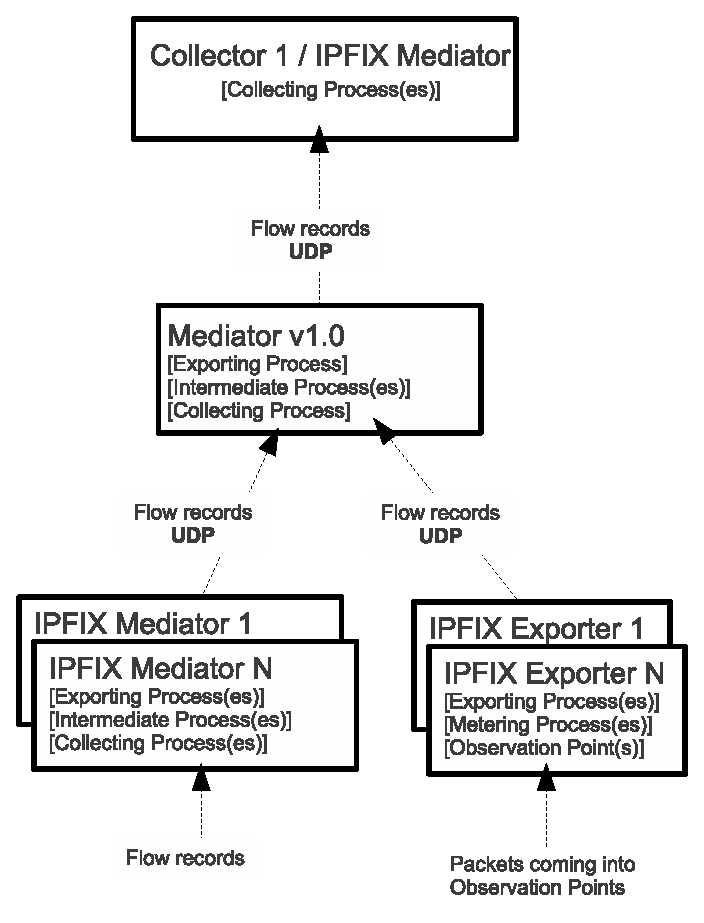
\includegraphics[width=0.5\textwidth]{kudla/eng_reference-model}
\caption{Mediator v1.0 reference model overview}\label{o:eng_reference-model}
\end{figure}

Basic \emph{Mediator v1.0} component model is shown in the Fig.~\ref{o:eng_mediator-components}. The 
Mediator may contain one or more Intermediate Processes hierarchically located between one Collecting and one
Exporting Process. 

Intermediate Processes are key functional blocks for IPFIX Mediation. Data flow between them is managed 
in the following ways:
\begin{itemize}
 \item \textbf{Parallel processing} - record stream is processed by Intermediate Processes simultaneously. 
 In this setup, each Intermediate Process receives a copy of the entire record stream as its input.
 \item \textbf{Serial processing} - In order to ensure flexible manipulation of a record stream, 
 the Intermediate Processes are connected serially. In that case, an output record stream from one 
 Intermediate Process forms an input for a~succeeding Intermediate Process.
\end{itemize}

   
\begin{figure}[ht!]
\centering
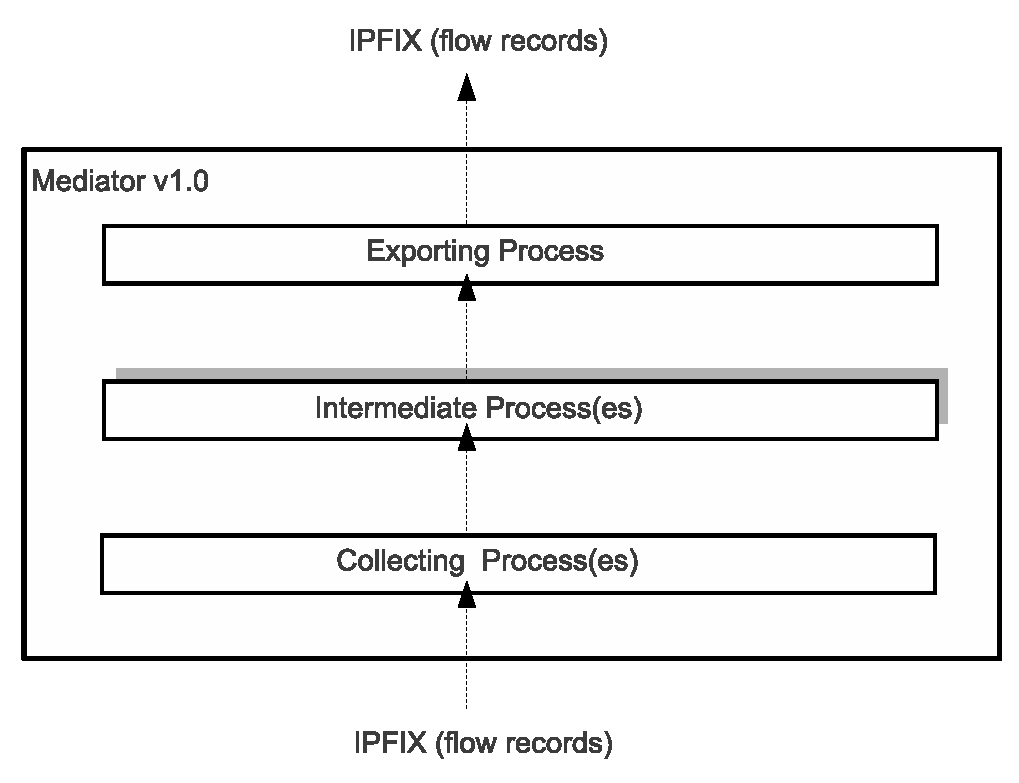
\includegraphics[width=0.6\textwidth]{kudla/eng_mediator-components}
\caption{Basic Mediator v1.0 component model}\label{o:eng_mediator-components}
\end{figure}

\subsection{Implementation of Mediator v1.0}

\subsubsection{Main class}

The role of the main class is to process command line arguments and then start all threads needed to run
the application. These threads are following: \emph{UDP Server}, \emph{UDP Processor}, \emph{UDP Exporter}
and each Intermediate 
Process is single thread as well. In case of error is Mediator shut down correctly so it releases memory and stops all 
running threads. Same situation occurs after pressing \verb|Ctrl-c|. 

\subsubsection{Collecting Process}

Logical structure of this process involves two stages, where each stage is one thread. 
Let us briefly describe the individual stages of the Collecting Process.

First stage is shown in Fig.~\ref{o:collecting1_schema}. A core class of this stage is \emph{UDPServer} 
which receives byte stream of IPFIX messages sent from Exporter over UDP protocol. This stream is wrapped 
into the \emph{PacketObject} and written to fast, blocking FIFO queue named \emph{PacketCache}. Application 
design allows for future extension with another transport protocols, such as TCP and SCTP. 

\begin{figure}[ht!]
\centering
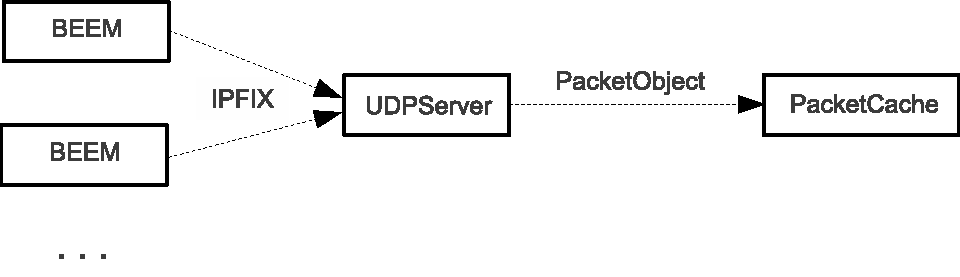
\includegraphics[width=0.7\textwidth]{kudla/collecting1_schema}
\caption{First stage of Collecting Process of Mediator v1.0}\label{o:collecting1_schema}
\end{figure}

Scheme of second stage depicts Fig.~\ref{o:collecting2_schema}. The UDP Processor thread works in cycle --
it reads packet objects from cache and sends them to IPFIX Parser. IPFIX Packets are split up there into
IPFIX message header, IPFIX template sets, data sets and options template sets. These entities are 
processed and transformed to flow records. IPFIX Parser sents each flow record with additional information 
to the class representing dispatcher of flow records -- \emph{FlowRecordDispatcher}. This class distributes 
received flow records to Intermediate Processes or send them to~the Exporting Process cache according to 
a configuration file.

\begin{figure}[ht!]
\centering
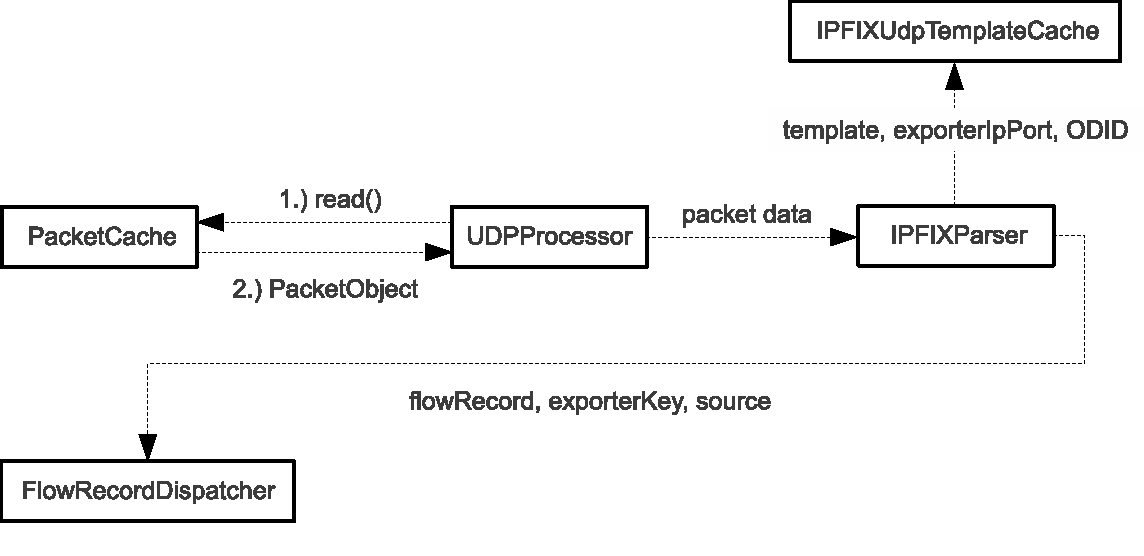
\includegraphics[width=0.8\textwidth]{kudla/collecting2_schema}
\caption{Second stage of Collecting Process of Mediator v1.0}\label{o:collecting2_schema}
\end{figure}

\subsubsection{Abstract class AIntermediateProcess}

This class is kind of an interface for Intermediate Processes (Modules) that separates their logic from framework
logic. Moreover, it defines basic characteristics of Modules and implements their methods. In other words 
-- it is parent class of each Intermediate Process.
Class provides following properties:
\begin{itemize}
 \item every Intermediate Process is single thread,
 \item every Intermediate Process has only one unique instance,
 \item decoding of data records,
 \item encoding of data records.
\end{itemize}

\subsubsection{Exporting Process}

A highest layer of Mediator v1.0 is the Exporting Process. Its scheme is shown in Fig.~\ref{o:eng_exporting-process}.
Core class -- UDP Exporter is a single thread and works in a cycle likewise UDP Processor and UDP Server. 
It reads flow records from FIFO queue named \emph{ExportCache} and sends them to message encoder, 
which creates IPFIX message byte stream. This stream is wrapped into UDP datagram and sent over computer 
network to an IPFIX Collector or another Mediator.

\begin{figure}[ht!]
\centering
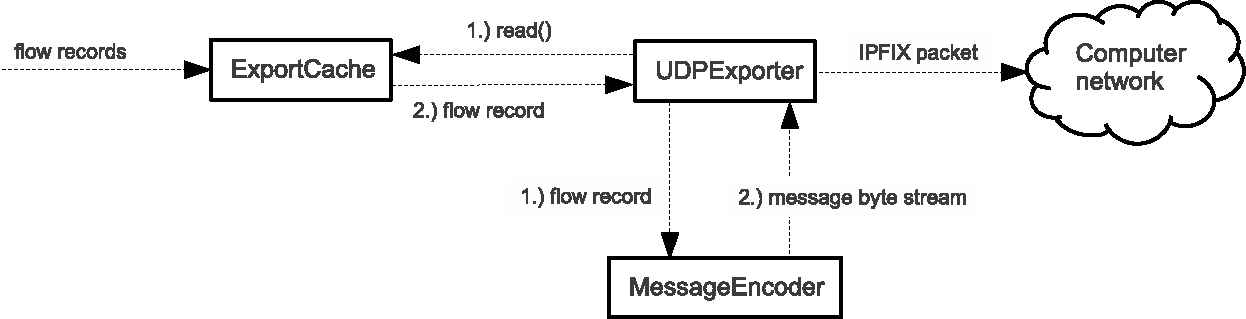
\includegraphics[width=0.9\textwidth]{kudla/eng_exporting-process}
\caption{Exporting Process scheme of Mediator v1.0}\label{o:eng_exporting-process}
\end{figure}

%% NEMENTE sekciu acknowledgement, ak vam vas veduci nepovie inak
\section{Acknowledgment}

This work is the result of the project implementation: Development of the Center of Information and 
Communication Technologies for Knowledge Systems (ITMS project code: 26220120030) supported 
by the Research \& Development Operational Program funded by the ERDF.

\section{Conclusion}

The main goal of this work was to design and implement framework for mediation entity (IPFIX Mediator)
between BEEM and JXColl in SLAmeter monitoring tool. Mediator v1.0 may greatly enhance measuring 
possibilities and flexibility of SLAmeter tool by hosting several Intermediate Processes. 

Accuracy of solution was confirmed by four experimental verifications. Future development
requires implementation of various Intermediate Processes. The greatest asset is seen in an anonymization
module and a selection module which will act as load-balancer among distributed Collectors. Module for 
conversion from NetFlow protocol to IPFIX might be important as well.





%% POZOR: AJ V ZOZNAME LITERATURY TREBA POUZIT MEDZINARODNE KODOVANIE
\begin{thebibliography}{4}
%
\bibitem{slameter}
MONICA research group: \emph{SLAmeter} [online], 2013. 
$<$\url{http://wiki.cnl.sk/Monica/SLAmeter}$>$.
%
\bibitem{rfc5982}
KOBAYASHI, A. -- CLAISE, B. et al.: \emph{IP Flow Information Export (IPFIX) Mediation: Problem Statement.} 
RFC 5982. 2010
%
\bibitem{rfc6183}
KOBAYASHI, A. et al.: \emph{IP Flow Information Export (IPFIX) Mediation: Framework.} 
RFC 6183. 2011
%
\bibitem{rfc5101}
CLAISE, B. et al.: \emph{Specification of the IP Flow Information Export 
(IPFIX) Protocol for the Exchange of IP Traffic Flow Information.} 
RFC 5101. 2008
%
\bibitem{rfc5470}
SADASIVAN, G. et al.: \emph{Architecture for IP Flow Information Export} 
RFC 5470. 2009

\end{thebibliography}

